\apendice{Especificación de diseño}
\section{Clasificación de las asignaturas}
Se ha realizado una clasificación general de las áreas a las que pertenecen de forma general las  asignaturas, de forma que se pueda mostrar un gráfico en la materia recomendable para un alumno. La siguiente tabla hace referencia a dicha clasificación \ref{tab:C.1}
\begin{table}[]
\caption{Tabla áreas educativas de las asignaturas }
\label{tab:C.1}
\resizebox{\textwidth}{!}{
\begin{tabular}{ lrrrrrrrr }
\toprule
 & Matemáticas & Derecho & Programación & Algoritmos & Idiomas & Economía & Diseño & Equipos informáticos \\  
\textbf{PRIMER SEMESTRE} &  &  &  &  &  &  &  &  \\  
Fundamentos Deontológicos y Jurídicos de las TIC & 1 & 1 & 0 & 0 & 0 & 0 & 0 & 0 \\  
Álgebra Lineal & 1 & 0 & 0 & 0 & 0 & 0 & 0 & 0 \\  
Informática Básica & 0 & 0 & 1 & 0 & 0 & 0 & 0 & 0 \\  
Fundamentos Físicos de la Informática & 1 & 0 & 0 & 0 & 0 & 0 & 0 & 0 \\  
Matemática Discreta & 1 & 0 & 0 & 0 & 0 & 0 & 0 & 0 \\  
\textbf{SEGUNDO SEMESTRE} &  &  &  &  &  &  &  &  \\  
Inglés Aplicado a la Informática & 0 & 0 & 0 & 0 & 1 & 0 & 0 & 0 \\  
Cálculo & 1 & 0 & 0 & 0 & 0 & 0 & 0 & 0 \\  
Programación & 0 & 0 & 1 & 1 & 0 & 0 & 0 & 0 \\  
Fundamentos de los Computadores & 0 & 0 & 1 & 0 & 0 & 0 & 0 & 1 \\  
Sistemas Operativos & 0 & 0 & 1 & 1 & 0 & 0 & 1 & 1 \\  
\textbf{TERCER SEMESTRE} &  &  &  &  &  &  &  &  \\  
Metodología de la Programación & 0 & 0 & 1 & 1 & 0 & 0 & 0 & 0 \\ 
Estadística & 1 & 0 & 0 & 0 & 0 & 0 & 0 & 0 \\ 
Ingeniería del Software & 0 & 0 & 0 & 0 & 0 & 0 & 1 & 0 \\  
Bases de Datos & 0 & 0 & 1 & 0 & 0 & 0 & 1 & 0 \\  
Arquitectura de Computadores & 0 & 0 & 1 & 0 & 0 & 0 & 0 & 1 \\  
\textbf{CUARTO SEMESTRE} &  &  &  &  &  &  &  &  \\  
Estructuras de Datos & 0 & 0 & 1 & 1 & 0 & 0 & 0 & 0 \\  
Redes & 0 & 0 & 0 & 0 & 0 & 0 & 0 & 1 \\  
Interacción Hombre-Máquina & 0 & 0 & 1 & 0 & 0 & 0 & 1 & 0 \\  
Fundamentos de Organización y Gestión de Empresas & 0 & 0 & 0 & 0 & 0 & 1 & 0 & 0 \\  
Análisis y Diseño de Sistemas & 0 & 0 & 0 & 0 & 0 & 0 & 1 & 0 \\  
\textbf{QUINTO SEMESTRE} &  &  &  &  &  &  &  &  \\ 
Arquitecturas Paralelas & 0 & 0 & 1 & 0 & 0 & 0 & 0 & 1 \\ 
Sistemas Inteligentes & 0 & 0 & 1 & 1 & 0 & 0 & 1 & 0 \\ 
Gestión de Proyectos & 0 & 0 & 1 & 0 & 0 & 1 & 1 & 0 \\ 
Diseño y Administración de Sistemas y Redes & 0 & 0 & 0 & 0 & 0 & 0 & 0 & 1 \\  
Procesadores del Lenguaje & 0 & 0 & 1 & 1 & 0 & 0 & 0 & 0 \\  
\textbf{SEXTO SEMESTRE} &  &  &  &  &  &  &  &  \\ 
Programación Concurrente & 0 & 0 & 1 & 0 & 0 & 0 & 0 & 1 \\  
Seguridad Informática & 0 & 1 & 1 & 1 & 0 & 0 & 0 & 1 \\ 
Aplicaciones de Bases de Datos & 0 & 0 & 1 & 0 & 0 & 0 & 1 & 1 \\  
Algoritmia & 0 & 0 & 1 & 1 & 0 & 0 & 0 & 0 \\ 
Métodos Numéricos y Optimización & 1 & 0 & 1 & 0 & 0 & 0 & 0 & 0 \\  
\textbf{SÉPTIMO SEMESTRE} &  &  &  &  &  &  &  &  \\  
Diseño e Implementación de Sistemas Digitales & 0 & 0 & 1 & 0 & 0 & 0 & 1 & 1 \\ 
Gestión de la Información & 1 & 0 & 1 & 1 & 0 & 1 & 0 & 0 \\ 
Diseño y Mantenimiento del Software & 0 & 0 & 1 & 0 & 0 & 0 & 1 & 0 \\  
Organización y Gestión de Empresas & 0 & 0 & 1 & 1 & 0 & 1 & 0 & 0 \\  
 Mantenimiento de Equipos Informáticos & 1 & 0 & 0 & 0 & 0 & 0 & 0 & 1 \\  
Hardware de Aplicación Específica & 0 & 0 & 1 & 0 & 0 & 0 & 1 & 1 \\ 
Control por Computador & 0 & 0 & 1 & 0 & 0 & 0 & 0 & 1 \\ 
Validación y Pruebas & 0 & 0 & 1 & 1 & 0 & 0 & 1 & 0 \\
Computación Neuronal y Evolutiva & 0 & 0 & 1 & 1 & 0 & 0 & 0 & 0 \\ 
Programación de Sistemas Operativos & 0 & 0 & 1 & 0 & 0 & 0 & 0 & 1 \\ 
\textbf{OCTAVO SEMESTRE} &  &  &  &  &  &  &  &  \\ 
Sistemas Distribuidos & 0 & 0 & 1 & 1 & 0 & 0 & 1 & 0 \\ 
Sistemas Empotrados y de Tiempo Real & 0 & 0 & 1 & 0 & 0 & 0 & 0 & 1 \\
Métodos Formales & 1 & 0 & 1 & 0 & 0 & 0 & 1 & 0 \\ 
Nuevas Tecnologías y Empresa & 0 & 0 & 1 & 1 & 0 & 0 & 0 & 0 \\ 
Minería de Datos & 1 & 0 & 1 & 1 & 0 & 0 & 0 & 0 \\ 
Desarrollo Avanzado de Sistemas Software & 0 & 0 & 1 & 0 & 0 & 0 & 1 & 0 \\ \bottomrule
\end{tabular}
}
\end{table}


\section{Modelo de Interfaz Gráfica}
La interfaz gráfica de escritorio de la primera versión se realizará con PyQt5, de forma que habrá varias ventanas diferentes dependiendo de la funcionalidad seleccionada: 
\subsection{Inicio de Sesión}
En la primera pestaña al ejecutar la aplicación, se mostraría la pantalla de inicio sesión para introducir el correo y la contraseña. La siguiente imagen hace referencia a un modelo básico de la pantalla de inicio de sesión. ~\ref{fig:C.2.1}
\begin{figure}[h]
\centering
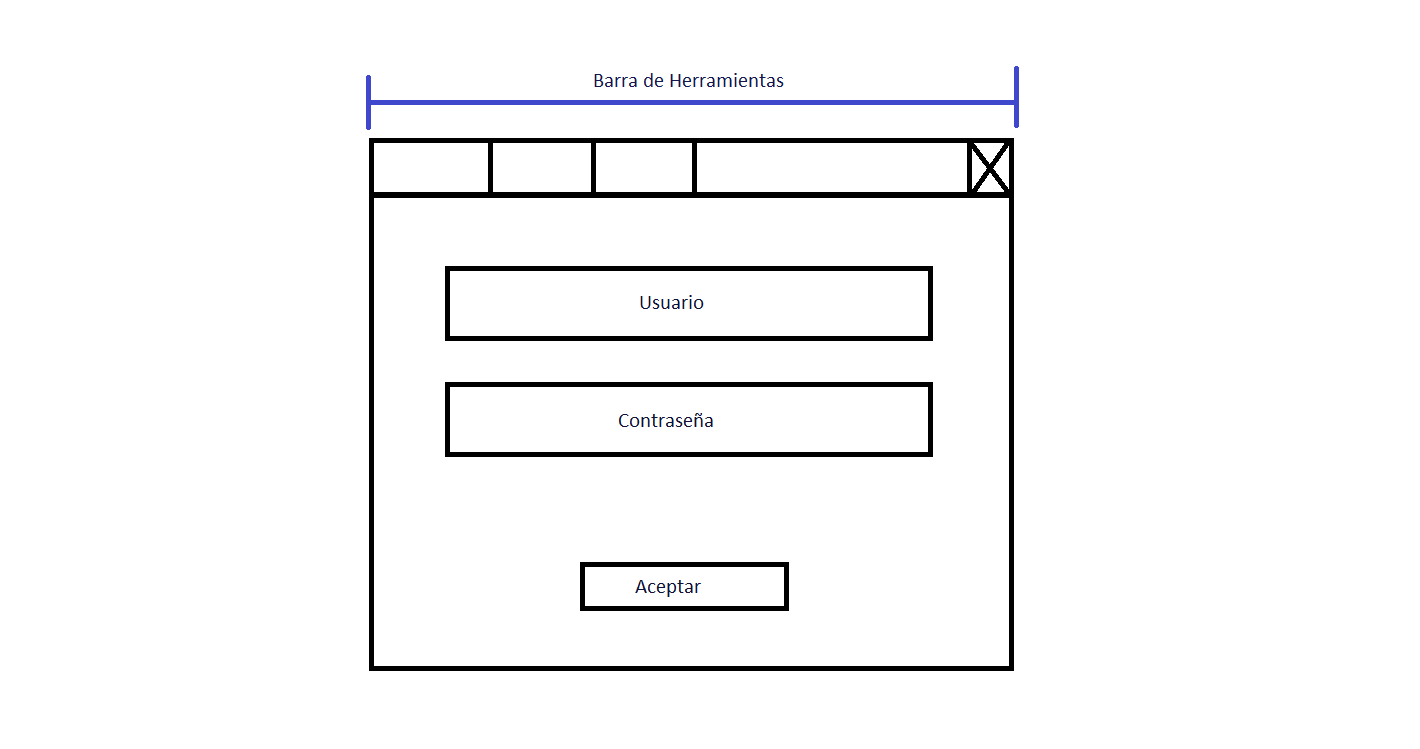
\includegraphics[width=0.90\textwidth]{PROTOTIPO_Inicio_sesion}
\caption{Prototipo de Inicio Sesión}
\label{fig:C.2.1}
\end{figure}

\subsection{Rellenado de cuestionario}
Una vez registrado por primera vez, un usuario debe rellenar el cuestionario con las ponderaciones de las asignaturas cursadas. Esta pestaña también sirve en caso de que el usuario se haya confundido en la calificación de alguna asignatura o repita el sistema de recomendación tras cursar nuevas asignaturas. Los diferentes cursos se seleccionarán en los botones para evitar un exceso de asignaturas mostradas en la pestaña. La siguiente imagen hace referencia a dicha pestaña. ~\ref{fig:C.2.2}
\begin{figure}[h]
\centering
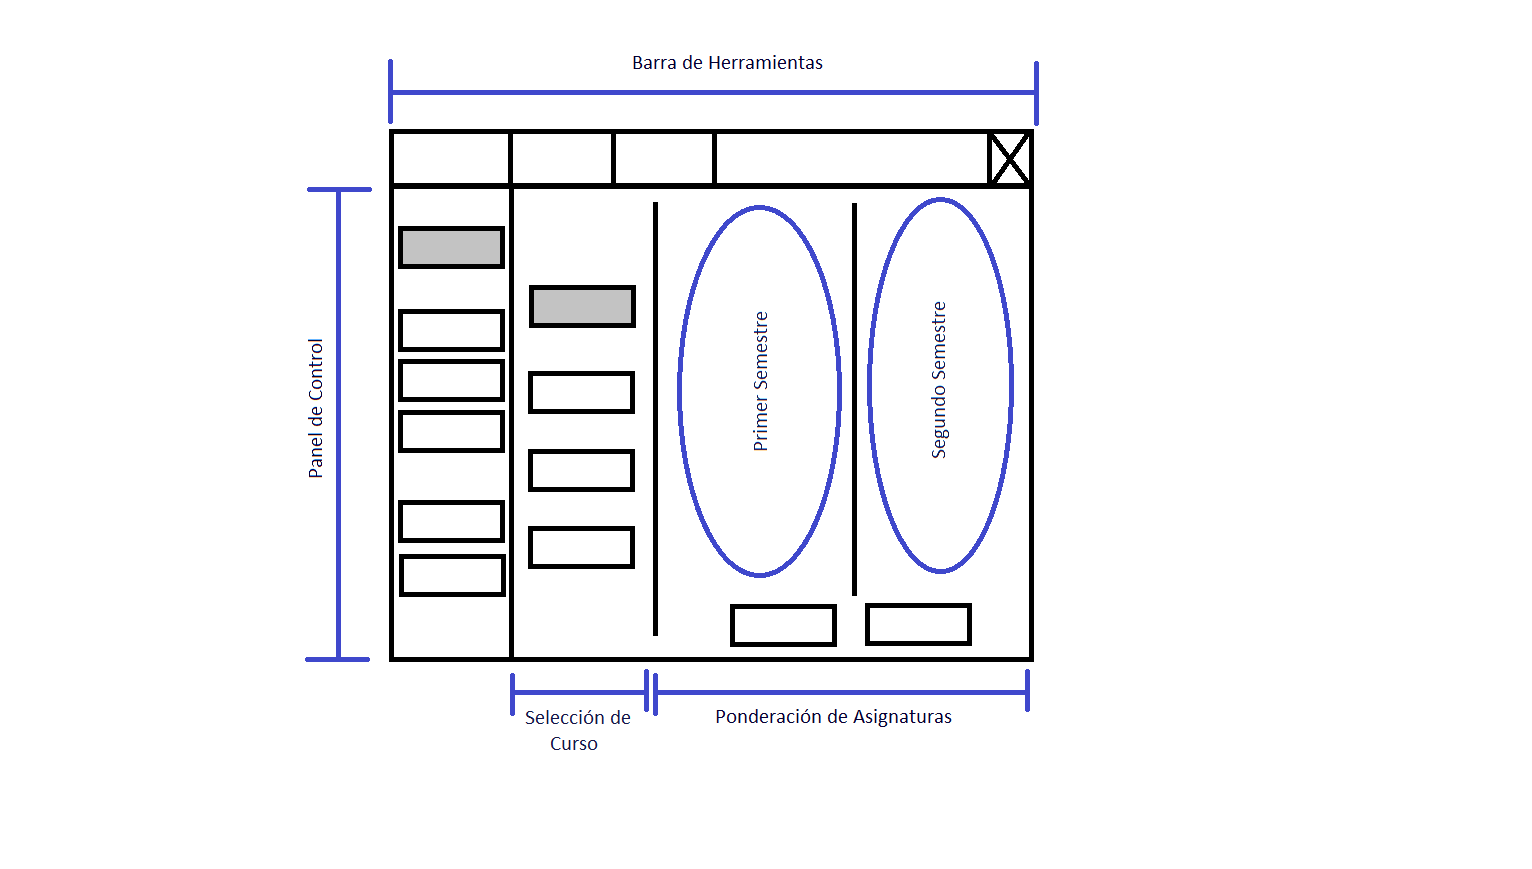
\includegraphics[width=0.90\textwidth]{PROTOTIPO_Rellenado_Datos}
\caption{Prototipo de Rellenado de datos}
\label{fig:C.2.2}
\end{figure}
\subsection{Muestra de resultados}
Tras rellenar el cuestionario para la recogida de datos, se seleccionará el sistema de recomendación deseado, y se mostrarán los resultados en base al sistema seleccionado, teniendo como patrón en el centro de la ventana los resultados de las asignaturas no cursadas, y en el tercio derecho, se mostrarán unas gráficas de las asignaturas y preferencias del alumno. La siguiente imagen hace referencia a dicha pestaña: ~\ref{fig:C.2.3}
\begin{figure}[h]
\centering
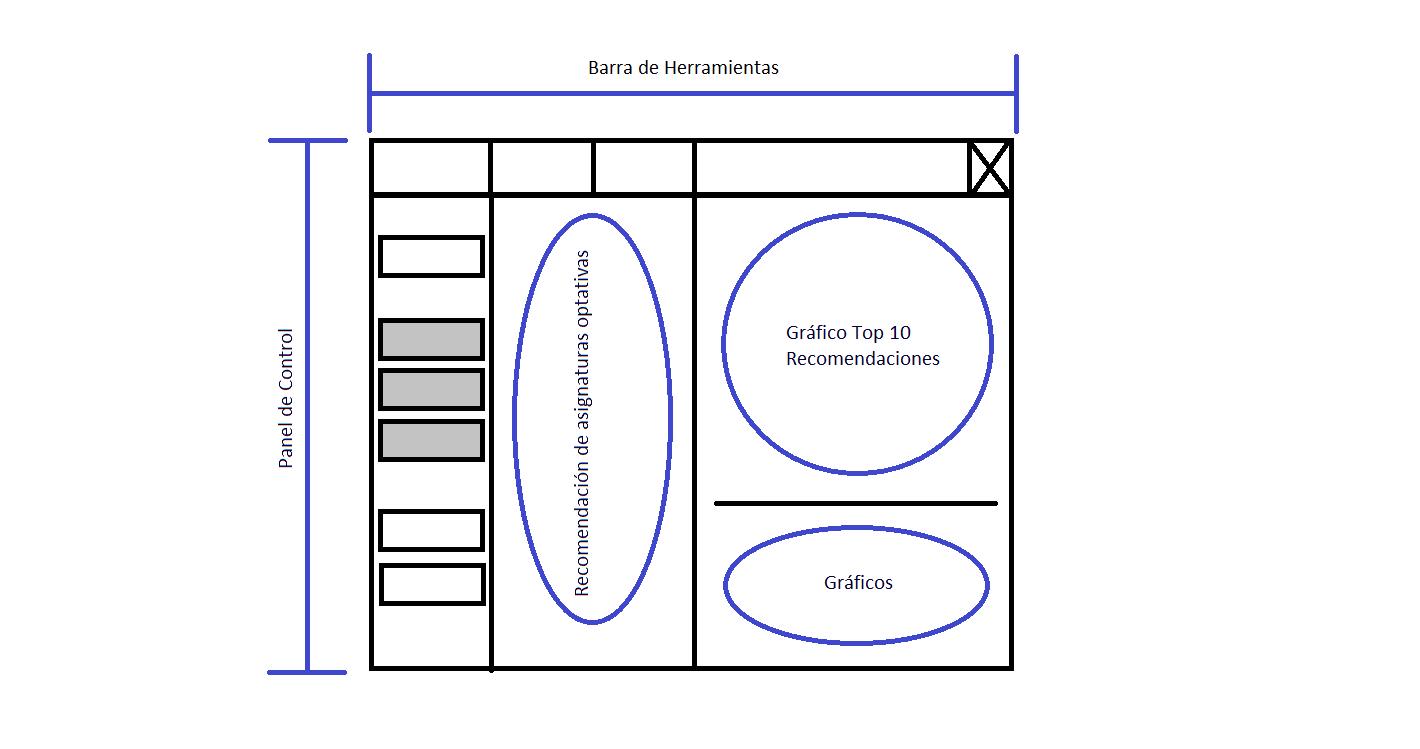
\includegraphics[width=0.90\textwidth]{PROTOTIPO_Sistemas_Recomendacion}
\caption{Prototipo de la muestra de datos}
\label{fig:C.2.3}
\end{figure}

\subsection{Otros datos}
Habrá un botón adicional que muestre las preferencias generales de media de los usuarios, así como otras gráficas para información adicional al usuario. 
La siguiente imagen hace referencia a dicha pestaña: ~\ref{fig:C.2.4}
\begin{figure}[h]
\centering
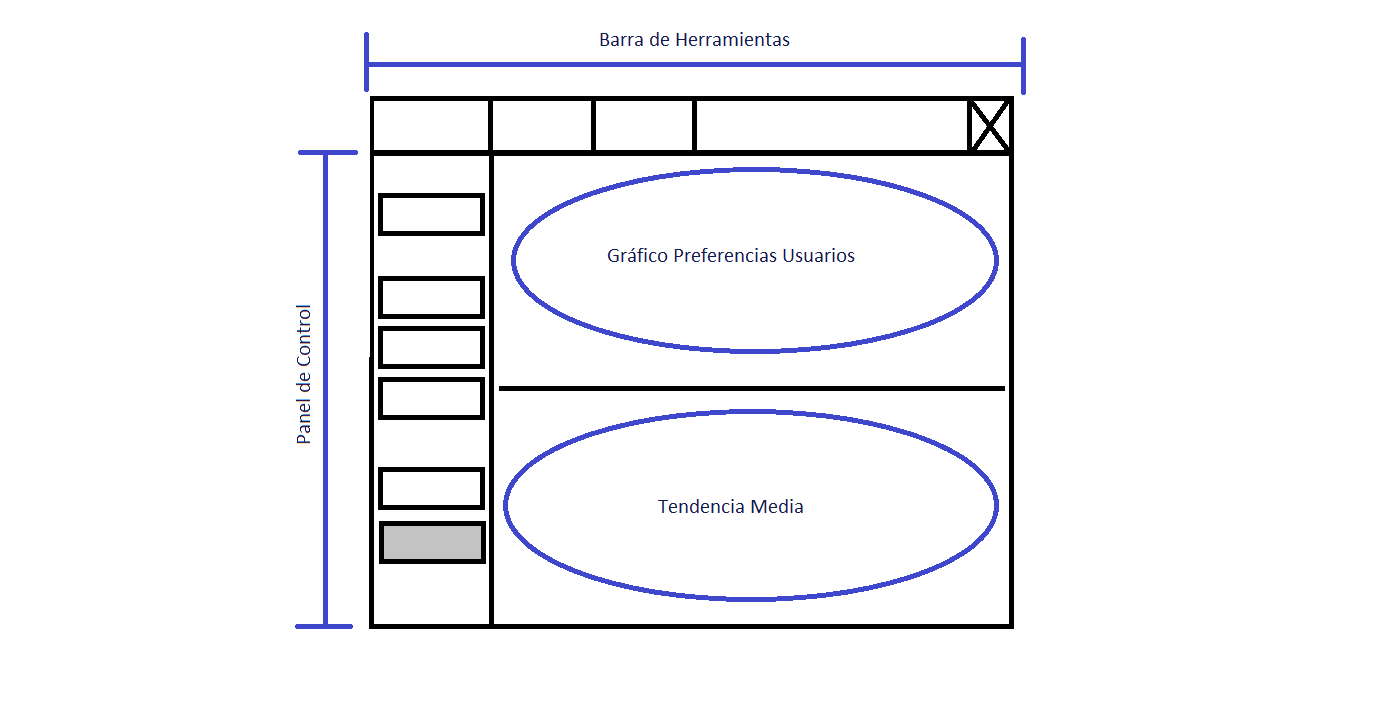
\includegraphics[width=0.90\textwidth]{PROTOTIPO_Otros_Datos}
\caption{Prototipo de datos adicionales}
\label{fig:C.2.4}
\end{figure}

\section{Diseño de Interfaz Gráfica }
\subsection{Inicio de Sesión}
La interfaz de inicio de sesión de la primera versión ~\ref{fig:C.3.1}  permite introducir el usuario y la contraseña en caso de estar registrado. En caso contrario, se debe pulsar "Registrarse" para crear una nueva cuenta. 
\begin{figure}[h]
\centering
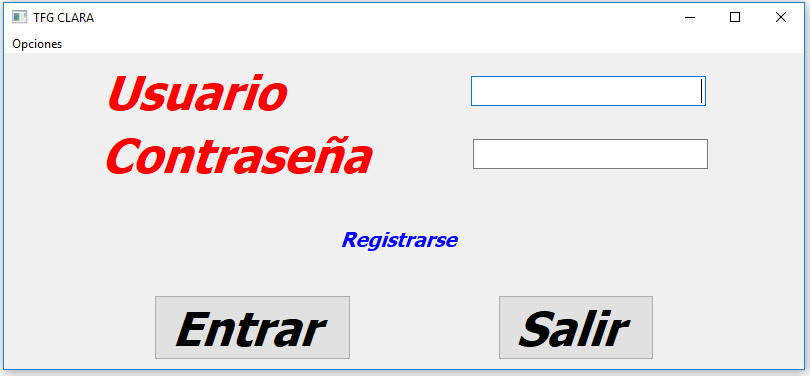
\includegraphics[width=0.90\textwidth]{INTERFAZ_Inicio_sesion}
\caption{Interfaz de inicio sesión}
\label{fig:C.3.1}
\end{figure}

\subsection{Rellenado de cuestionario}
\subsubsection{Versión 1.0}
Tras iniciar sesión, se mostrará la siguiente pestaña ~\ref{fig:C.3.2} en la que el usuario debe ponderar las asignaturas cursadas, siendo las del primer curso obligatorias para la ejecución del sistema de recomendación. 
\begin{figure}[h]
\centering
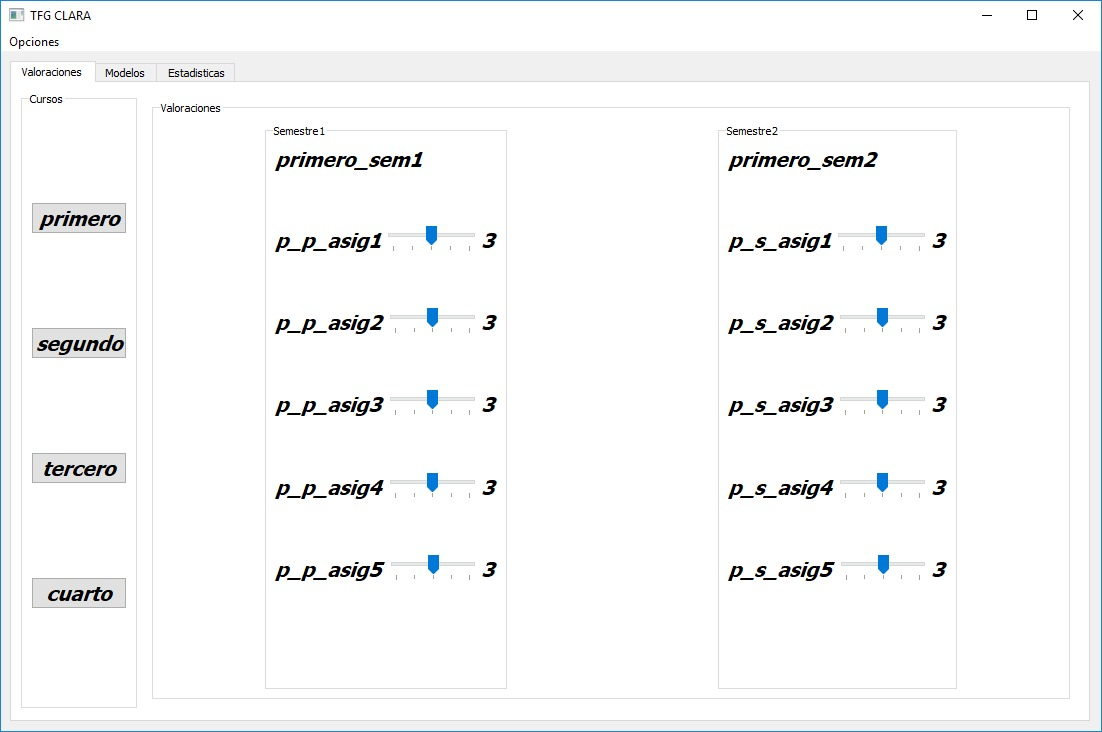
\includegraphics[width=0.90\textwidth]{INTERFAZ_Rellenado_Datos}
\caption{Interfaz de rellenado de cuestionario}
\label{fig:C.3.2}
\end{figure}

\subsubsection{Versión 1.1}
En la versión actualizada, se permite al usuario seleccionar las asignaturas como ``omitida'' para indicar que no se ha cursado dicha asignatura por convalidación. Esto se puede observar en la siguiente imagen: ~\ref{fig:C.3.3.1}
\begin{figure}[h]
\centering
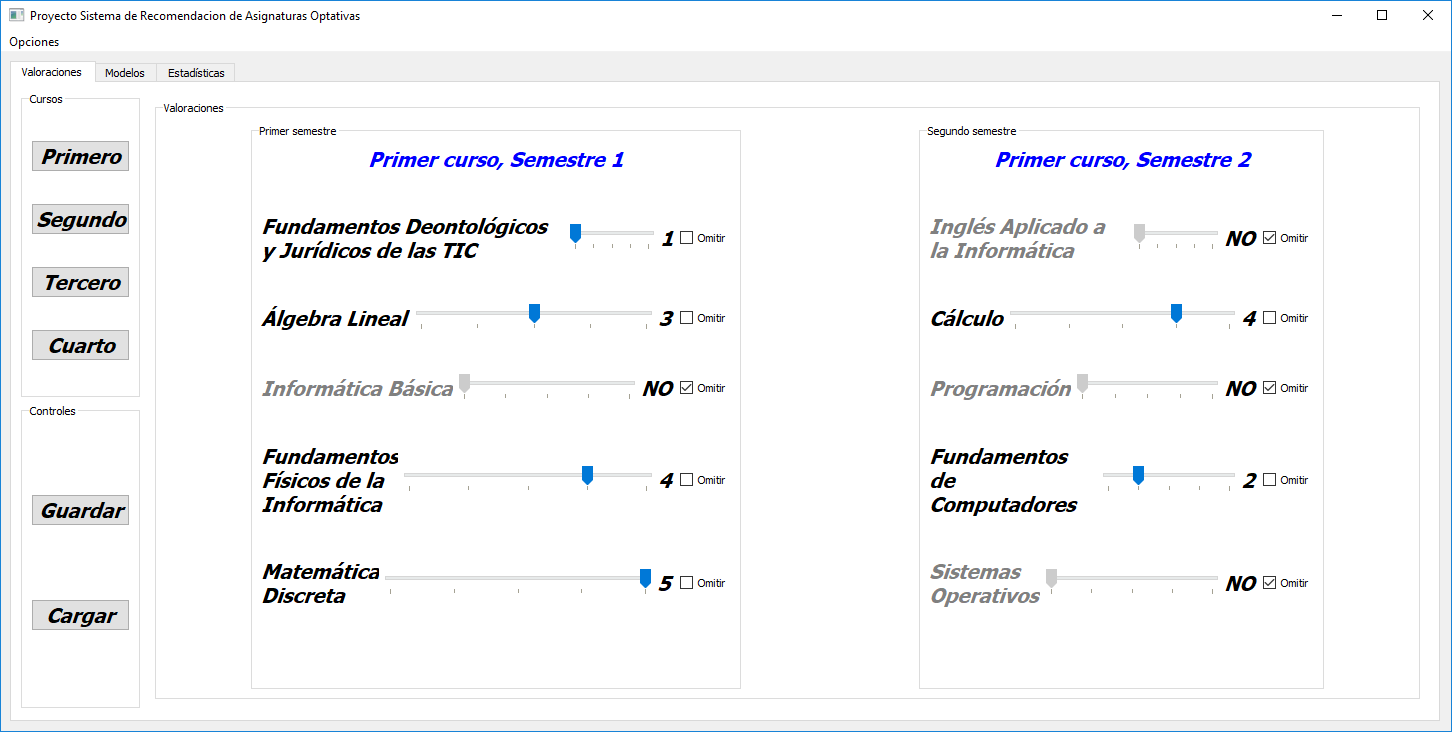
\includegraphics[width=0.90\textwidth]{INTERFAZ_1_1_Principal}
\caption{Interfaz de rellenado de cuestionario final}
\label{fig:C.3.3.1}
\end{figure}

\subsection{Muestra de resultados}
Tras el rellenado de datos, se habilitan los botones de la selección del sistema de recomendación, mostrándose una pestaña similar a la siguiente: ~\ref{fig:C.3.3}
\begin{figure}[h]
\centering
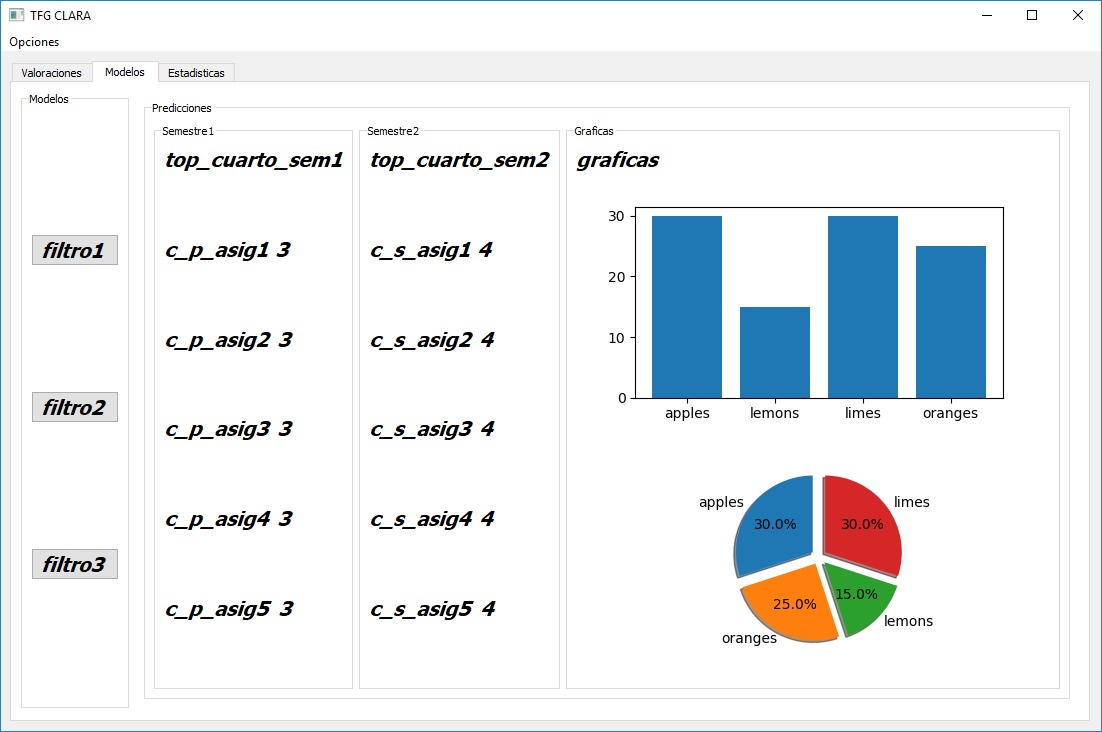
\includegraphics[width=0.90\textwidth]{INTERFAZ_Sistemas_Recomendacion}
\caption{Interfaz de la muestra de datos}
\label{fig:C.3.3}
\end{figure}

\subsection{Otros datos}
\subsubsection{Versión 1.0}
Se le mostrará unos datos auxiliares al usuario, en forma de gráficas, para mejorar su comprensión. Esto corresponde a la tercera pestaña de la aplicación. ~\ref{fig:C.3.4}
\begin{figure}[h]
\centering
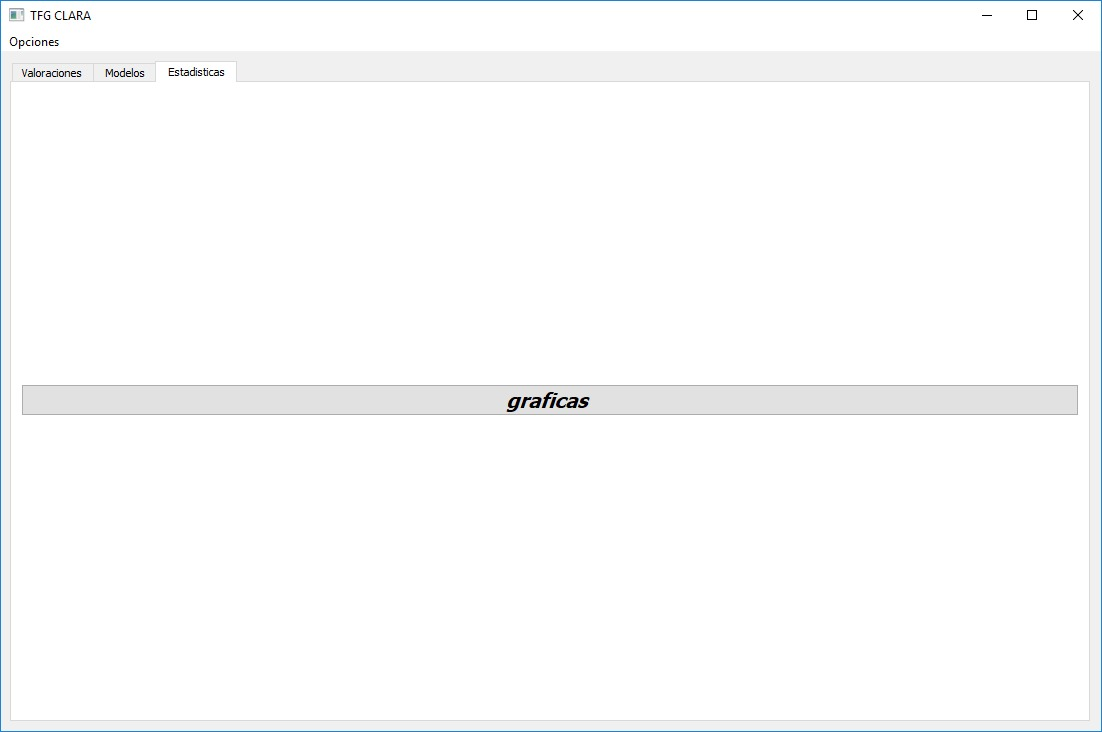
\includegraphics[width=0.90\textwidth]{INTERFAZ_Otros_datos}
\caption{Interfaz de datos adicionales}
\label{fig:C.3.4}
\end{figure}
\subsubsection{Versión 1.1}
La versión entregable de la tercera pestaña muestra datos de interés para el usuario. Correspondería con la siguiente imagen:~\ref{fig:C.3.4.1}
\begin{figure}[h]
\centering
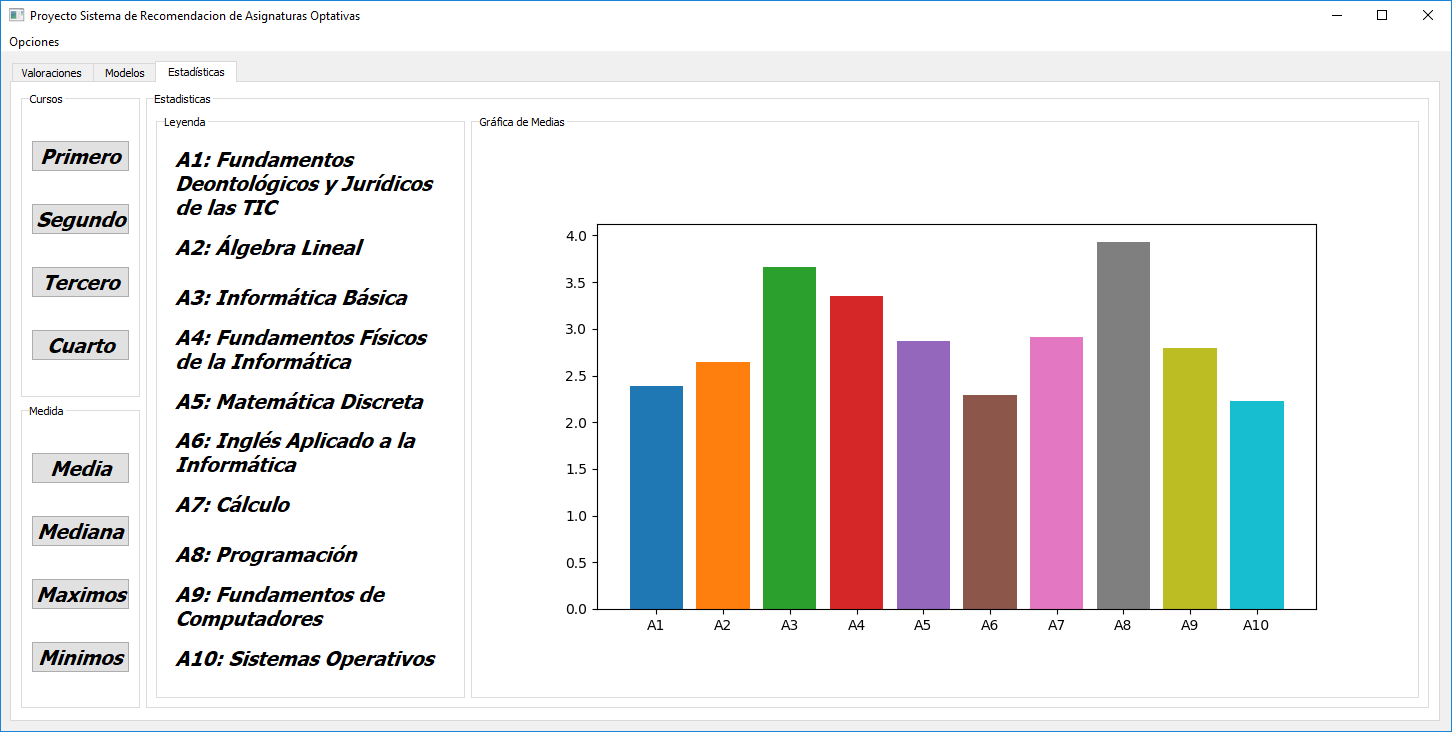
\includegraphics[width=0.90\textwidth]{INTERFAZ_Estadistica}
\caption{Interfaz de datos adicionales}
\label{fig:C.3.4.1}
\end{figure} 
En ella se permitirá observar las medias, medianas, máximos y mínimos de las calificaciones generales de los usuarios. De esta forma, al usuario se le informa de la opinión general del resto de estudiantes con respecto a dicha asignatura. 
\section{Posibles acciones del Usuario}
A continuación se detallarán las posibles acciones que se le permite realizar a un usuario: 
\subsection{Pestaña de Inicio}
En la pestaña de inicio, se permite a un usuario: 
\begin{itemize}
\item \textbf{Registrarse}: Al registrarse,-recibiendo el rol de Usuario y nunca de Admin- se le solicitará: 
\begin{itemize}
\item Nombre
\item Correo
\item Contraseña
\end{itemize}	

\item \textbf{Iniciar Sesión}: Al iniciar sesión se le solicitará  al usuario el usuario y la contraseña, validándose que los datos sean correctos.
\item \textbf{Salir}: Al pulsar el botón salir, se cerrará la pestaña, al igual si pulsa la X de la esquina superior derecha. 
\item \textbf{Aceptar}: Tras rellenar correctamente Usuario y Contraseña, se pulsará el botón aceptar para iniciar sesión y acceder a la aplicación. 
\end{itemize}


\subsection{Rellenado de Datos}
El primer botón de la pestaña superior permite acceder al rellenado de los datos para obtener las calificaciones de las asignaturas no cursadas. En caso de no haberse rellenado el mínimo necesario de las asignaturas, el resto de los botones, en la pestaña de selección del sistema de recomendación, exceptuando "Salir" permanecerán desactivados.  A partir de la versión 1.1, la versión entregable al tribunal, se permite no aplicar unas determinadas asignaturas para no ser utilizadas en los sistemas de recomendación. 
La interacción que se le permite al usuario en dicha pestaña será la siguiente. 
\begin{itemize}
\item \textbf{Selección del curso}: Selección del curso para rellenar los datos. 
\item \textbf{Ponderación de asignatura}: Se permite ponderar en un Slider tanto con el ratón, como con el teclado.
\item \textbf{Guardar}: Guardar los datos insertados  manualmente  por el usuario. 
\item \textbf{Modificación}: Se permitirá al usuario modificar las calificaciones en caso de haber insertado incorrectamente la ponderación. 
\item \textbf{Anulación}: Se permitirá al usuario no aplicar una determinada asignatura que haya convalidado para no ser calculada en el sistema de recomendación. 
\end{itemize}

\subsection{Selección del sistema de Recomendación}
La selección del sistema de recomendación se realiza en la segunda pestaña de la aplicación. En dicha pestaña, habrá botones que  estarán deshabilitados hasta que el usuario complete el rellenado mínimo de los datos. 
La interacción que se le permite-tras habilitarse-será la siguiente: 
\begin{itemize}
\item \textbf{Selección del sistema de recomendación}:Seleccionar el cálculo de un determinado sistema de recomendación. 
\item \textbf{Visualización del orden de asignaturas}: Ver el orden de la asignatura en la gráfica, colocando el ratón sobre la asignatura. 
\end{itemize}

\subsection{Muestra de otros datos}
La tercera pestaña hacer referencia  a la muestra de datos al usuario. Para ello, en un principio, no se le añadirá funcionalidad auxiliar al usuario.
Al usuario se le permite: 
\begin{itemize}
\item \textbf{Calcular}: Seleccionar el cálculo deseado (Media, Mediana, Máximo y Mínimo)
\item\textbf{Selección del curso}: Seleccionar el curso para ver los valores de las asignaturas. 
\item \textbf{Cerrar}: Cerrar la pestaña. 
\end{itemize}

\section{Posible diseño de Clases} 
El paquete Core,  en el que se encontrará toda la estructura de los sistemas de recomendación, se subdivide en dos paquetes diferentes: I\_O (de entrada y salida de datos) y Filtros (para el desarrollo de los sistemas de recomendación). La siguiente imagen corresponde con dicho esquema. 
 ~\ref{fig:C.3.5}
\begin{figure}[h]
\centering
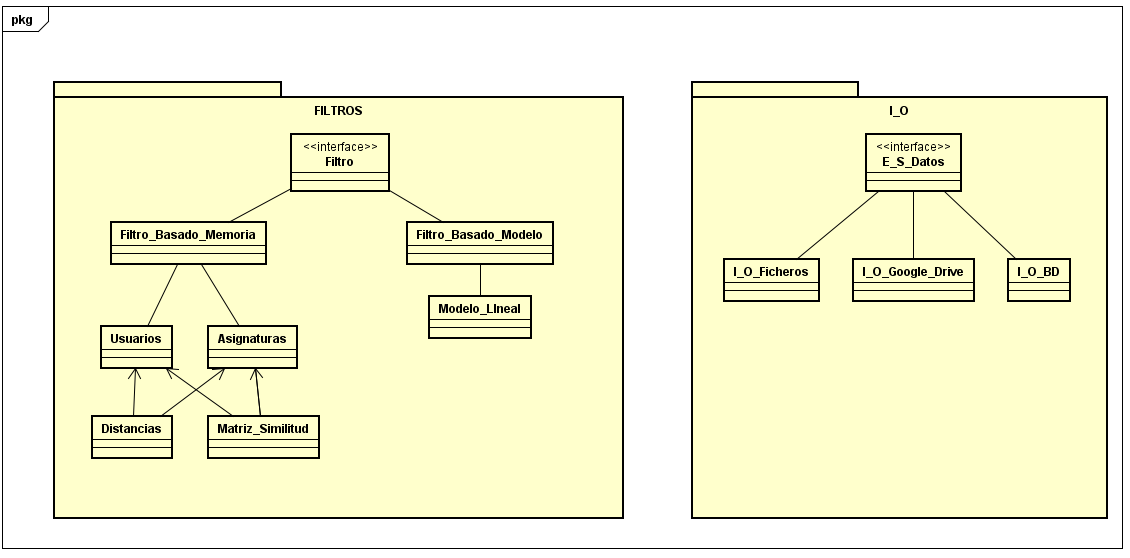
\includegraphics[width=0.90\textwidth]{Diagrama_Core}
\caption{Diagrama de Clases del Core}
\label{fig:C.3.5}
\end{figure}
El paquete GUI, por su parte, contendrá la estructura de la interfaz gráfica, para permitir la interacción del usuario con los sistemas de recomendación de forma ágil. La siguiente imagen hace referencia a dicho esquema.  ~\ref{fig:C.3.6}
\begin{figure}[h]
\centering
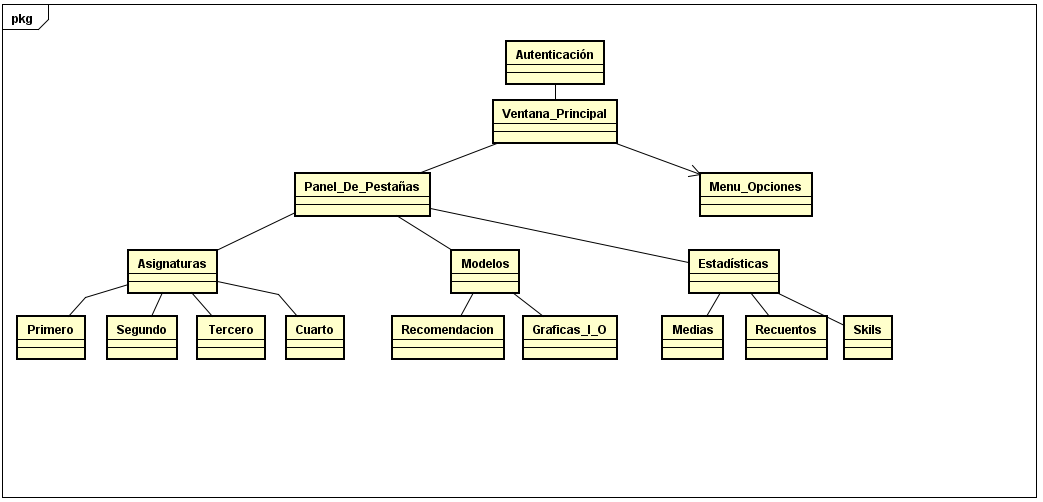
\includegraphics[width=0.90\textwidth]{Diagrama_Interfaz}
\caption{Diagrama de Clases del GUI}
\label{fig:C.3.6}
\end{figure}
\subsubsection{Paquete Core}
El paquete Core almacena dos paquetes en su interior: 
\begin{itemize}
\item \textbf{Filtro}: El paquete filtro contienen todo el código necesario para el desarrollo de los diferentes sistemas de recomendación. A su vez, este paquete contiene en su interior: 
\begin{itemize}
\item F\_B\_Memoria: Este paquete contendrá en su interior el desarrollo de los sistemas de recomendación con Filtro colaborativo basado en Memoria. 
\begin{itemize}
\item Productos: Este paquete contendrá la clase para el desarrollo del  Filtro colaborativo basado en Productos, clase que recibe la tabla de datos, y la matriz de similitud para ejecutar el sistema. 
\item Usuarios : Este paquete contendrá la clase para el desarrollo del filtro colaborativo basado en Usuarios, clase que recibe la tabla de datos y la matriz de similitud, ambos datos recibidos del paquete Util. 
\item Util: Este paquete desarrolla la matriz de distancias y la matriz de similitud en dos clases diferentes para  su utilización en los filtros colaborativos basados en memoria.  
\end{itemize}
\item F\_B\_Modelos: Este paquete aún no ha sido desarrollado. 
\end{itemize}
\item \textbf{I\_O}: Este paquete I\_O desarrollará las entradas y salidas de datos, tanto por fichero, por bases de datos y por GoogleDrive. De esta forma:
\begin{itemize}
\item I\_I\_O\_Datos: Implementará la entrada y salida de datos desde Base de Datos. 
\item I\_O\_Datos\_Binario: Implementa la entrada y salida de los desde-a fichero binario. 
\item I\_O\_Datos\_GoogleDrive: Clase que implementa la entrada y transformación de los datos anónimos recogidos en Google Drive para el entrenamiento de los sistemas de recomendación y su almacenamiento en Base de Datos. 
\end{itemize} 
\end{itemize}

\subsubsection{Paquete GUI}
El paquete GUI almacena el código para el desarrollo del la interfaz gráfica para la interacción con el usuario. Este paquete contiene en su interior: 
\begin{itemize}
\item \textbf{Autenticación}: Este paquete contiene en su interior la clase de inicio sesión, para introducir el usuario y la contraseña para ejecutar la aplicación. A su vez, dicho paquete contiene: 
\begin{itemize}
\item VentanaPrincipal: El paquete VentanaPrincipal contiene la clase para mostrar el esqueleto de lo que será la ventana que se muestre tras iniciar sesión. A su vez, dicho paquete contendrá en su interior dos paquetes e para el desarrollo de  las pestañas y las opciones de la interfaz. 
\begin{itemize}
\item Panel\_De\_Pestañas : Este paquete contiene las clases para desarrollar la interfaz gráfica con la que interactuará el usuario. 
\begin{itemize}
\item Asignaturas: Este paquete contiene las clases para almacenar los nombres de las asignaturas, así como los cursos para realizar las ponderaciones. Este paquete hace referencia a la primera pestaña.   
\item Estadisticas: El paquete Estadística contiene los datos para el desarrollo de las estadísticas de la aplicación. 
\item Modelos: Este paquete implementa las clases y métodos para mostrar el Top 10 de los sistemas de recomendación para las asignaturas de cuarto curso y la muestra de los resultados. 
\end{itemize}

\item Menu\_Opciones: Este paquete contiene la implementación del cerrado de la página. 
\end{itemize}
\end{itemize}
\end{itemize}
\section{Diseño Procedimental}
Los diferentes pasos para el correcto funcionamiento de la aplicación son los siguientes: 
\subsection{Recogida de datos}
En este apartado no se ha realizado una programación propiamente dicha. Se ha utilizado typeform para la creación del cuestionario anónimo. con el siguiente enlace: \url{https://clarapalacios.typeform.com/to/RQRRfY}
La portada del cuestionario es la siguiente. 
~\ref{fig:D.1.1}
\begin{figure}[h]
\centering

\includegraphics[width=0.90\textwidth]{cuestionario_anonimo_inicio}
\caption{Imagen inicial del cuestionario}
\label{fig:D.1.1}
\end{figure}
Por otra parte, el usuario final de la aplicación en un principio no tiene por qué rellenar dicho cuestionario, ya que ha sido creado con el único fin de recopilar datos. 
Tras la recopilación de datos, éstos se almacenarán en Drive, en un documento Excel. 
\subsection{Almacenamiento y recuperación de los datos}
La recuperación de los datos en Python desde GoogleDrive se permite gracias a la librería oauth2client y se almacena bien en un fichero binario, bien en la base de datos. 
Este procedimiento no es visto por el usuario final, al igual que la recogida de datos, de forma que una vez iniciada sesión, los datos ya se habrán cargado en la primera pestaña. 

\subsection{Inicio sesión}
Un usuario cualquiera, se registra en la aplicación-en caso de ser su primer acceso-o inicia sesión, accediendo a las ponderaciones rellenadas del grado.  Tras pulsar aceptar, accede a la pestaña principal de rellenado y modificación de datos.

\subsection{Rellenado de datos}
En caso de haberse registrado, la pestaña principal con el rellenado de asignaturas por curso permanecerá con una ponderación básica en todas las asignaturas (1), así como las asignaturas del cuarto curso permanecerán deshabilitadas, pudiéndose modificar por el usuario tanto por teclado como con el ratón. Por otro lado, se permite habilitar o deshabilitar una asignatura para no ser contabilizada por el sistema de recomendación.  
 
\subsection{Cálculo del sistema de recomendación}
Tras el rellenado de los datos, en la segunda pestaña, se le permite al usuario seleccionar el sistema de recomendación deseado, calculándose los valores de las asignaturas no cursadas y mostrándose dicho cálculo por pantalla. Los sistemas de recomendación no ejecutados por el usuario permanecerán desactivados. 
\subsection{Muestra de Gráficos Auxiliares}
La tercera pestaña mostrará gráficos y datos de interés para el usuario con respecto a las asignaturas cursadas y ponderadas por otros usuarios. 


\section{Diagrama de Clases Final}
Este proyecto cuenta con dos partes: 
\subsection{Autenticación}
La autenticación consta de un paquete src con una única clase, utilizada para almacenar y recuperar los datos de la base de datos (tanto los datos de las asignaturas como del usuario. 
Al haber problemas con las inserciones de asignaturas con espacios y tildes, se han tenido que traducir dichas asignaturas para poder almacenarlas en la BD. ~\ref{fig:C.4.1}
\begin{figure}[h]
\centering
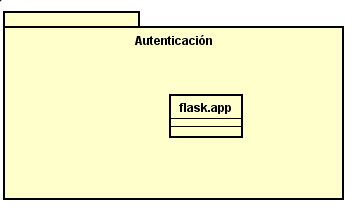
\includegraphics[width=0.90\textwidth]{Diagrama_Autenticacion}
\caption{Diagrama de Clases de la Autenticación}
\label{fig:C.4.1}
\end{figure}
Hay que tener en cuenta que no se debe confundir dicho paquete con el incluido en GUI, el cual 

\subsection{Sistema de recomendación de Asignaturas Optativas}
En el sistema de recomendación, al igual que en la primera versión, los paquetes se subdividen en GUI,  Core y Dicc. Actualmente, dichos paquetes se encuentran incluidos en un paquete Proyecto, de forma que todos los paquetes se encuentren centralizado  en una única carpeta. Los paquetes GUI y Core permanecen invariables según lo que se ha realizado en la primera versión, mientras que se ha modificado el paquete del diccionario. 
\subsubsection{Dicc}
El paquete Dicc contiene el diccionario de traducción para la interfaz gráfica, de forma que no haya que introducir las cadenas de texto en el código, y se evite la repetición de las mismas. Este paquete contiene en su interior: 
\begin{itemize}
\item Dicc: Diccionario para la traducción de los botones, cabeceras y áreas de la interfaz gráfica. Esto permite, en caso de introducir un nuevo lenguaje, no necesitar reescribir el cógido, sino introducir un nuevo diccionario de las variables. 
\item NombreAsignaturas: Esta clase contiene los getter y setter de las asignaturas de la carrera, así como el establecimiento de los diccionarios de los semestres y la caracterización de las asignaturas para obtener el campo sobre el que se desarrollan. 
\end{itemize}
La estructura de clases de dicho paquete es la siguiente: ~\ref{fig:C.4.2}
\begin{figure}[h]
\centering
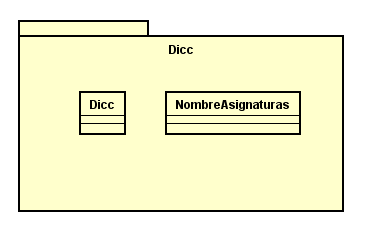
\includegraphics[width=0.90\textwidth]{Diagrama_Dicc}
\caption{Diagrama de Clases del Diccionario}
\label{fig:C.4.2}
\end{figure}
